\documentclass[a4paper]{iacas}

\usepackage{cite}
\usepackage{hyperref}% embedding hyperlinks [must be loaded after dropping]
\usepackage{amsmath,amsthm,amssymb,amsfonts,latexsym,mathrsfs,wasysym}
\usepackage{marvosym}
\usepackage{subcaption}
\usepackage{soul,color}
\usepackage{threeparttable}% tables with footnotes
\usepackage{dcolumn}% decimal-aligned tabular math columns
\usepackage{float}
\usepackage{graphicx}
\usepackage{accents}
\usepackage{tikz}
\usepackage{lastpage}
\usepackage{fancyhdr}
\usepackage{color}
\usepackage{cancel}
\usepackage{setspace}
%\doublespacing
% or:
\onehalfspacing
%\usepackage[T1]{fontenc}
%\usepackage{bigfoot} % to allow verbatim in footnote
\usepackage[framed,numbered]{matlab-prettifier}
\pagestyle{plain}
%\usepackage[hebrew,english]{babel}
\usetikzlibrary{shapes.geometric, arrows, calc}

\newcolumntype{d}{D{.}{.}{-1}}
\graphicspath{{figures/}}

% define some commands to maintain consistency
\newcommand{\pkg}[1]{\texttt{#1}}
\newcommand{\cls}[1]{\textsf{#1}}
\newcommand{\file}[1]{\texttt{#1}}
\newcommand{\sgn}[1]{\operatorname{sgn}\left(#1\right)}
\newcommand{\sat}[1]{\operatorname{sat}\left(#1\right)}
\newcommand{\rrule}[1]{\rule[#1]{0pt}{0pt}}
\newcommand{\fracds}[2]{\frac{\displaystyle #1\rrule{-0.2em}}{\displaystyle #2\rrule{1em}}}
\newcommand{\figref}[1]{Fig.~\ref{#1}}
\newcommand{\ubar}[1]{\underaccent{\bar}{#1}}
\newcommand{\norm}[1]{\lvert \lvert \vec #1 \rvert \rvert}

%diffeomorphism

\begin{document}

\begin{center}
 \large Algorithms and Application in Computer Vision - 046746
 \end{center}
\begin{center}
\large\textbf{Homework \#1}
 \end{center}


\begin{tabular}{l}
\\
{\bf\textit{Alexander Shander}} \\
{\bf\textit{Vladimir Tchuiev 309206795}} \\
Technion - Israel Institute of Technology
\end{tabular}

\vspace{2em}

\section{Part 2}

\subsection{Part 2b}

The default format for image data in Matlab is \textbf{uint8}. This format does not support negative numbers that result from subtraction of image data matrices (all $L_l[I]$ except for $l=n$), thus when reconstructing back the original image the reconstruction is not accurate (Fig~\ref{fig:rec1b}) and results in a bloom effect. To solve this problem, the image data needs to be converted to \textbf{double}, thus supporting negative values. This allows for an accurate reconstruction (Fig~\ref{fig:rec2b}).

\begin{figure}[!htbp]
	
	\begin{subfigure}[b]{0.48\textwidth}
		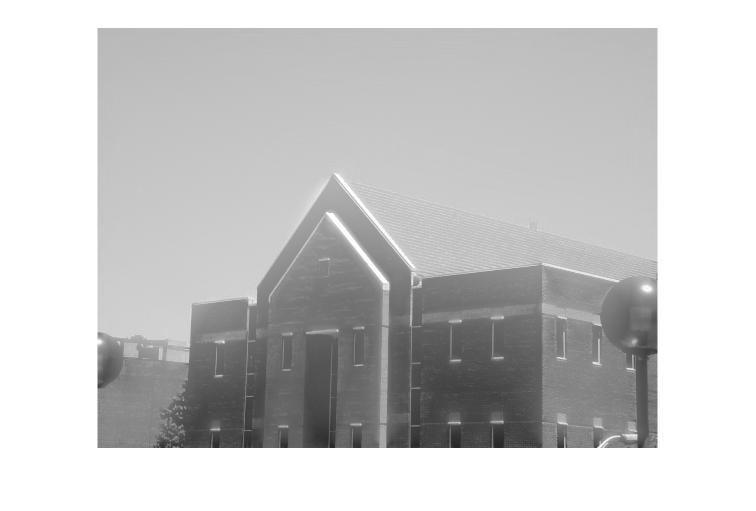
\includegraphics[width=\textwidth]{rec_1_building.jpg}
		\caption{}
		\label{fig:rec1b}
	\end{subfigure}
	%
	\begin{subfigure}[b]{0.48\textwidth}
		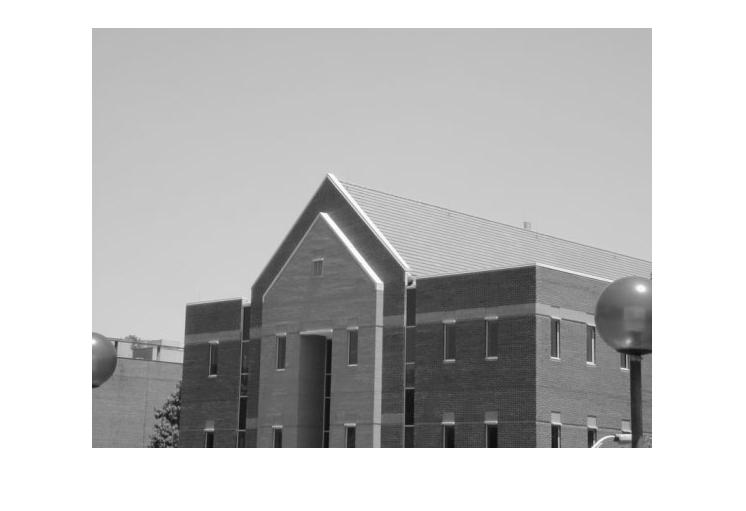
\includegraphics[width=\textwidth]{rec_2_building.jpg}
		\caption{}
		\label{fig:rec2b}
	\end{subfigure}
	
	\caption{\textbf{(a)}: recreated image from uint8 laplacian pyramid. \textbf{(b)}: recreated image from double laplacian pyramid}
	
\end{figure}

\end{document}
